\cotefile{145}

\scanpage{28}
dans $\mathcal E$, qu'on peut choisir canoniquement en prenant le quart de grand cercle qui joint $P$ au milieu $2$ du \deleted{segment} l'arc $(1,\infty)$ de grand cercle opposé à $0$, ce qui définit un isom du rev. universel de $U$ en $P$, avec celui de $U$ en $\bar P$ sur lequel le groupe précédent opère de façon canonique, donc aussi par transport de structure sur $\tilde U\deleted{\unsure{(\overline P)|(\mathcal E)}}_{\deleted{\unsure{\mathcal E|\xi}}}(P)$, donc il s'envoie dans $\mathcal E$.

On trouve que
\[
\dot\sigma_0\mapsto\sigma_0,\quad\dot\tau\to\tau_0
\]
est le remontage correspondant. De $=$ pour le pt fixe $-1$ de $\dot\sigma_1$, ou $\frac12$ de $\dot\sigma_\infty$, on trouve des scindages partiels sur les ss-groupes de \deleted{\unsure{conj.}} stabilité $\Gamma_{-1}\subset\Gamma$ et $\Gamma_2\subset\Gamma$. Il est commode de poser
\[
\deleted{\unsure{\Gamma|F}}\quad 2=0',\quad -1=1',\quad \tfrac12=\infty',
\]
d'où des groupes d'isotropie $\Gamma_{0'}=\{\dot\sigma_0,\tau\}$, $\Gamma_{1'}=\{\dot\sigma_1,\tau\}$, et $\Gamma_{\infty'}=\{\dot\sigma_\infty,\tau\}$, qui se remontent resp en $\sigma_0$ et $\tau_0$, \unsure{en|ou} $\sigma_1$ et $\tau_1$, en $\sigma_\infty$ et $\tau_\infty$.

Les composantes connexes de $U^\tau$ sont les trois arcs de grand cercle entre $0,1,\infty$, qui contiennent chacun un \deleted{pt} et un seul des pts $0',1',\infty'$, et les classes de conjugaison
\mspage{27}

\scanpage{29}
\mspage{13}
correspondantes de relèvements \inserted{de $\{1,\dot\tau\}$} sont resp. les relèvements en $\tau_0$, en $\tau_1$ et en $\tau_\infty$ --- qui ne donnent rien de nouveau. Reste à considérer $\tau\dot\sigma_1$ (et ses conjugués \inserted{par $\rho$} $\tau\dot\sigma_\infty$, $\tau\dot\sigma_0$), on a $\dot\sigma_1(2)=1/2$, donc
\[
(\tau\dot\sigma_1)(2)=\frac12
\]
et
\[
U^{\tau\dot\sigma_1}=\{z\in U\mid z\bar z=1\}=\mathbb U-\{1\},
\]
où $\mathbb U=\{z\in\mathbb C\mid|z|=1\}$. Cet ensemble contient $P$ et $\bar P$, et ne donne donc pas de nouveaux \unsure{relèvements|relèvement} p.r. à celui déjà donné, avec $\tilde\sigma_1$ relevant $\dot\sigma_1\tau$.

\unsure{Il|Je} faudrait quand-$\bar m$ donner aussi une description de $\mathcal E$ tt entier par gén. et relations, en partant d'un syst. de gén. de $\Gamma=\unsure{\mathfrak S_3|\mathcal S_3}\times\mathbb Z/2$, qu'on va relever de façon judicieuse. On prendra les \inserted{quatre} générateurs
\[
\deleted{\displaystyle
\deleted{\unsure{\rho'|\dot\rho'}}=\rho\unsure{\tau|\deleted{\tau}},\quad\deleted{\unsure{\tau}}\underset{\substack{\Vert\\\dot\sigma_0\tau}}{\widetilde{\dot\sigma}_0},\quad\underset{\substack{\Vert\\\dot\sigma_1\tau}}{\widetilde{\dot\sigma}_1},\quad\underset{\substack{\Vert\\\dot\sigma_\infty\tau}}{\widetilde{\dot\sigma}_\infty},
}
\]
\deleted{
\inserted{(donc ${\rho'}^6=1$, ${\rho'}^3=\tau$, ${\rho'}^2=\rho^2=\rho^{-1}$)}
avec les relations
}
\[
\deleted{\displaystyle
\left\{\begin{aligned}
\widetilde{\dot\sigma}_1^2&=\widetilde{\dot\sigma}_2^2=\widetilde{\dot\sigma}_3^2=1\\
\widetilde{\dot\sigma}_0\widetilde{\dot\sigma}_1&=\widetilde{\dot\sigma}_1\widetilde{\dot\sigma}_\infty=\widetilde{\dot\sigma}_\infty\widetilde{\dot\sigma}_0=\unsure{{\rho'}^{\deleted{-1}2}|\dot\rho^{-2}}\\
{\rho'}^6&=1\\
{\rho'}^3&\text{ commute aux }\dot\sigma_i
\end{aligned}\right.
}
\]
\mspage{28}

\scanpage{30}
\deleted{qui décrivent $\unsure{\mathfrak S_3|\mathcal S_3}\times\mathbb Z/2$, on va relever ces générateurs en des \unsure{élts|éléments} de $\mathcal E$, de façon que $l_\infty,l_1,l_0$ s'expriment comme des mots en ces \unsure{élts|éléments}, et il suffit alors d'ajouter cette relation $l_\infty l_1l_0$ aux relations correspondant aux précédentes\ldots}

$\dot\sigma_0,\dot\sigma_1,\dot\sigma_\infty,\unsure{\dot\rho|\rho},\tau$, avec les relations
\[
\left\{\begin{aligned}
\dot\sigma_0^2&=\dot\sigma_1^2=\dot\sigma_\infty^2=1\\
\dot\sigma_0\dot\sigma_1&=\dot\sigma_1\dot\sigma_\infty=\dot\sigma_\infty\dot\sigma_0=\dot\rho\\
\dot\rho^3&=1\\
\tau^2&=1\\
\tau&\text{ commute à }\dot\sigma_0,\dot\sigma_1,\dot\sigma_\infty\quad\text{(donc aussi à }\dot\rho\text{)}
\end{aligned}\right.
\]
on les relève en $\deleted{\tau_0,\tau_1,\tau_\infty}\ \sigma_0,\sigma_1,\sigma_\infty,\rho,\underbrace{\tau_0,\tau_1,\tau_\infty}_{\text{sur }\tau}$ avec les relations
\[
\left\{\begin{aligned}
\sigma_0^2&=\sigma_1^2=\sigma_\infty^2=\tau_0^2=[\tau_1^2=\tau_\infty^2]=1\\
\rho^3&=1\\
\rho\tau_0\rho^{-1}&=\tau_1,\quad\rho\tau_1\rho^{-1}=\tau_\infty,\quad\rho\tau_\infty\rho^{-1}=\tau_0\\
\tau_0\sigma_{\unsure{0|\infty}}&=\sigma_0\tau_0,\quad\tau_1\sigma_1=\sigma_1\tau_1,\quad\tau_\infty\sigma_\infty=\sigma_\infty\tau_\infty\\
\sigma_0\sigma_1&=\tau_\infty\tau_1\rho,\quad\sigma_1\sigma_\infty=\tau_0\tau_\infty\rho,\quad\sigma_\infty\sigma_0=\tau_1\tau_0\rho
\end{aligned}\right.
\]
\margin{NB Il faut ajouter les relations
\[
\left\{\begin{aligned}
\rho\sigma_0\rho^{-1}&=\sigma_1\\
\rho\sigma_1\rho^{-1}&=\sigma_\infty\\
\rho\sigma_\infty\rho^{-1}&=\sigma_0
\end{aligned}\right.
\]
sont conséquences des relations ci-contre}
\margin{Ce sont les \unsure{éléments|élémts} $\tilde\sigma_0,\tilde\sigma_1,\tilde\sigma_\infty$ $\longrightarrow$}
\margin{[NB On trouve
\[
\begin{gathered}
l_0=\tau_\infty\tau_1,\quad\deleted{l_1=\tau_0\tau_\infty},\\
l_1=\tau_0\deleted{\unsure{l_\infty=}}\tau_\infty\\
l_\infty=\tau_1\tau_0
\end{gathered}
\]
et $l_\infty l_1l_0=1$ est automatique]}
\margin{$\uparrow$ \deleted{\unsure{Or|On|Ceci}} Ceci indique que $\tau_0,\tau_1,\tau_\infty$ \unsure{conjuguent|engendrent} \unsure{un|le} ss-groupe engendré par $l_0,l_1,l_\infty$}

\deleted{\uline{Question} \deleted{\uline{\unsure{Peut-on}}}\inserted{On peut} exprimer $\rho$ en fonction de $\sigma_0,\sigma_1,\sigma_\infty,\tau_0,\tau_1,\tau_\infty$ ??, \deleted{\unsure{et pas plus}}\inserted{par l'une des} \unsure{dernier|derniers} \unsure{groupe|groupes} de relations, et substituer dans les autres.}
\mspage{29}

\scanpage{31}
\mspage{14}
On peut prendre aussi comme seuls gén. $\rho,\sigma_0,\tau_0$ (dont se déduisent $\sigma_1,\tau_1$, \inserted{$\sigma_\infty,\tau_\infty$,} comme $\rho\sigma_0\rho^{-1},\rho\tau_0\rho^{-1},\rho^2\sigma_0\rho^{-2},\rho^2\tau_0\rho^{-2}$) et les relations
\[
\left\{\begin{aligned}
\text{i)}\quad&\sigma_0^2=\tau_0^2=1\quad\tau_0\sigma_0=\sigma_0\tau_0\quad\text{(i.e. }(\overbrace{\sigma_0\tau_0}^{\tilde\sigma_0})^2=1\text{)}\\
\text{b)}\quad&\rho^3=1\\
&\sigma_0\underbrace{\rho\sigma_0^{-1}\rho^{-1}}_{\sigma_1}=\underbrace{\rho^2\cdot\tau_0\rho^{-2}}_{\tau_\infty}\underbrace{\rho\tau_0\rho^{-1}}_{\tau_1}\rho\\
&\text{i.e. }\sigma_0\rho\sigma_0^{-1}\rho^{-1}=\rho^{-1}\tau_0\rho\tau_0\\
&\text{ou enfin }\rho\sigma_0\rho^{-1}\sigma_0=\tau_0\rho^{-1}\tau_0\rho\quad\text{soit}\\
&\text{soit}\quad[\rho,\sigma_0][\rho^{-1},\tau_0]=1
\end{aligned}\right.
\]
\margin{\unsure{\deleted{i.e.}|i.e.} ou encore $\deleted{\operatorname{int}(\rho)\sigma_0}\quad[\rho,\sigma_0]=[\tau_0,\rho^{-1}]$}

C'est donc un quotient du produit libre $(\mathbb Z/2\mathbb Z\times\mathbb Z/2\mathbb Z)*\mathbb Z/3\mathbb Z$, par le sous-groupe invariant décrit par la relation $[\rho,\sigma_0][\rho^{-1},\tau_0]=1$.

\uline{NB} On trouve une symétrie dans le groupe, qui échange $\sigma_0$ et $\tau_0$, et échange $\rho$ et $\rho^{-1}$. [donc qui échange aussi $\sigma_1$ et $\tau_\infty$, $\sigma_\infty$ et $\tau_1$] --- mais cette symétrie n'est pas compatible avec la structure d'extension, comme on voit de \deleted{\unsure{s}} de suite (en\unsure{:|;} en passant au quotient $\unsure{\mathfrak S_3|\mathcal S_3}\times\mathbb Z/2$, elle devrait conserver le centre!).
\mspage{30}

\scanpage{33}
\mspage{\unsure{15|13}}
\textcircled{2} \uline{Le groupe} $S\widehat{\widehat{\mathcal E}}$.

Par le calcul, il s'explicite comme l'ens des systèmes
\[
(1)\qquad\left(\underset{\hat{\mathbb Z}^{*}}{\underset{\rotatebox{-90}{$\in$}}{p}},\underset{\unsure{\mathfrak S_3|\mathcal S_3}}{\underset{\rotatebox{-90}{$\in$}}{\sigma}},\underset{\hat\pi}{\underset{\rotatebox{-90}{$\in$}}{g_0}},\underset{\hat\pi}{\underset{\rotatebox{-90}{$\in$}}{g_1}},\underset{\hat\pi}{\underset{\rotatebox{-90}{$\in$}}{g_\infty}}\right)=\tilde u
\]
satisfaisant la condition
\[
(2)\qquad\operatorname{int}(g_{\deleted{\unsure{0}}\infty})(l_{\sigma(\infty)}^p)\cdot\operatorname{int}(g_1)(l_{\sigma(1)}^p)\cdot\operatorname{int}(g_{\unsure{\infty|0}})(l_{\sigma(\unsure{\infty|0})}^p)=1
\]
et tels que les trois facteurs de ce produit soient un syst. de générateurs de $\hat\pi$ [avec la relation génératrice (2)]. Le morphisme $u$ défini par ce \deleted{morphi} système est
\[
(3)\qquad\left\{\begin{aligned}
u(l_0)&\deleted{\mapsto}=\operatorname{int}(g_0)l_{\sigma(0)}^p\\
u(l_1)&=\operatorname{int}(g_1)l_{\sigma(1)}^p\\
u(l_\infty)&=\operatorname{int}(g_\infty)l_{\sigma(\infty)}^p
\end{aligned}\right.
\]
\inserted{ce qui explicite l'hom can}
\[
(4)\qquad S\widehat{\widehat{\mathcal E}}\xrightarrow{p}\widehat{\widehat{\mathcal E}}=\operatorname{Aut}_{\unsure{\mathrm{lac}|\mathrm{loc}}}(\hat\pi)
\]
L'homomorphisme canonique
\[
(5)\qquad i:\hat\pi\times\hat{\mathbb Z}^{\{0,1,\infty\}}\longrightarrow S\widehat{\widehat{\mathcal E}}
\]
s'explicite par
\[
(6)\qquad i(g;\alpha_0,\alpha_1,\alpha_\infty)=(1,1,gl_0^{\alpha_0},gl_1^{\alpha_1},gl_\infty^{\alpha_\infty})
\]
donc
\[
(7)\quad\deleted{\text{donc}}\quad pi(g;\alpha_0,\alpha_1,\alpha_\infty)=\operatorname{int}g.
\]
\margin{On retrouve que \unsure{(4)|(p)} est surjectif, et a comme noyau $i(\hat\pi)$}
La multiplication dans $\widehat{\widehat{\mathcal E}}$ est donnée par
\[
(8)\quad\underbrace{(p,\sigma,g_0,g_1,g_\infty)}_{\tilde u}\underbrace{(p',\sigma',g'_0,g'_1,g'_\infty)}_{\tilde u'}=(pp',\sigma\sigma',u(g'_0)g_{\sigma'(0)},u(g'_1)g_{\sigma'(1)},u(g'_\infty)g_{\sigma'(\infty)}\unsure{)}
\]
Cette formule n'est pas, du point de vue du calcul\unsure{,}
\mspage{32}

\scanpage{34}
entièrement explicite et \unsure{satisfaisante|satisfaisant}, puisque au deuxième membre interviennent les quantités $u(g'_0),u(g'_1),u(g'_\infty)$, qui ne sont donc pas exprimées directement en termes des \inserted{\unsure{seules|formelles}} données $(p,\sigma,g_0,g_1,g_\infty)$, $(p',\sigma',g'_0,g'_1,g'_\infty)$; \deleted{\unsure{sauf}}\inserted{mais ils s'explicitent ainsi} quand $g'_0,g'_1,g'_\infty$ sont eux-mêmes donnés explicitement comme des mots (ou limites de tels) en les $l_0,l_1,l_\infty$.

Cependant quand $\tilde u$ est de la forme $i(g,\alpha_0,\alpha_1,\alpha_\infty)$, on trouve (en laissant tomber les $'$ du 2e facteur)
\[
(9)\quad i(g,\alpha_0,\alpha_1,\alpha_\infty)(p,\sigma,g_0,g_1,g_\infty)=(p,\sigma,\deleted{\unsure{\operatorname{int}}}gg_0l_{\unsure{\sigma0|\sigma(0)}}^{\alpha_{\sigma(0)}},gg_1l_{\sigma1}^{\alpha_{\sigma(1)}},gg_\infty l_{\sigma\infty}^{\alpha_{\unsure{\sigma(\infty)}}})
\]
qui se simplifie pour $\sigma=1$ en
\[
(9')\quad i(g,\alpha_0,\alpha_1,\alpha_\infty)(p,1,g_0,g_1,g_\infty)=(p,\sigma,gg_0l_0^{\alpha_0},gg_1l_1^{\alpha_1},gg_\infty l_\infty^{\alpha_\infty})
\]
Par ailleurs, l'opération de $\widehat{\widehat{\mathcal E}}$ sur $i(\pi\times\mathbb Z^{\{0,1,\infty\}})$ par autom int. s'explicite aisément, et ne dépend que de $u$ \deleted{et}\unsure{:|.}
\[
(10)\quad\tilde u\,i(g;\alpha_0,\alpha_1,\alpha_\infty)\unsure{\deleted{u}\inserted{\tilde u^{-1}}|\tilde u^{-1}}=i(u(g);p\alpha_{\sigma^{-1}0},p\alpha_{\sigma^{-1}1},p\alpha_{\sigma^{-1}\infty})
\]
où $\tilde u=(p,\sigma;g_0,g_1,g_\infty)$

--- mais sur cette formule, on peut faire les mêmes commentaires que plus haut, sur le manque d'explicitation du \unsure{terme|\deleted{2ième}|\deleted{2ème}} $u(g)$ de cette formule, pour $g$ non exprimé comme un mot \unsure{p.r.|p.v.} aux $l_0,l_1,l_\infty$ (ou limite de tels mots)
\mspage{33}

\scanpage{35}
\mspage{16}
On va regarder de plus près la partie $S\hat{\mathcal E}$ de $S\widehat{\widehat{\mathcal E}}$, image inverse de
$\underset{\substack{\Vert\\\hat\Gamma}}{\Gamma}=\unsure{\mathfrak S_3|\mathcal S_3}\times\mathbb Z/2\unsure{\subset|\in|\leftarrow}\widehat{\widehat\Gamma}=\operatorname{Autext}_{\unsure{\mathrm{lac}|\mathrm{loc}}}\hat\pi$\unsure{,|.}

On va regarder les éléments $
% Unidentified canceled sign drawn from scan; no letter assigned.
\deleted{\unsure{\vcenter{\hbox{\tikz[x=0.7em,y=0.7em,baseline=0pt]{\draw[line width=0.45pt] (0.12,0.92)--(0.05,0.72)--(0.19,0.48)--(0.22,0.16); \draw[line width=0.45pt] (0.08,0.72)--(0.35,0.86) (0.13,0.53)--(0.36,0.67) (0.20,0.22)--(0.08,0.10); \draw[line width=0.65pt] (0.32,0.27)--(0.46,0.22)--(0.44,-0.06);}}}}}\rho,\deleted{\unsure{\tau}},\dot\sigma_0,\sigma_1,\sigma_\infty,\tau_0,\tau_1,\tau_\infty$ de $\widehat{\widehat{\mathcal E}}$, \deleted{\unsure{extérieurs|secteurs}} (NB. ils sont $\bar m$ dans $\mathcal E$) et voir comment ils se relèvent en $S\widehat{\widehat{\mathcal E}}$ (et $\bar m$, en $S\mathcal E$). En fait, par $\dot\rho\mapsto\rho,\dot\sigma_0\mapsto\tilde\sigma_0=\sigma_0\tau_0$, on a un relèvement \inserted{multiplicatif} de $\Gamma_P^*=\{(\sigma,\operatorname{sg}(\sigma))\mid\sigma\in\unsure{\mathfrak S_3|\mathcal S_3}\}$ dans $\mathcal E$, qu'on aimerait remonter à $S\mathcal E$ --- et de $\bar m$ pour $\dot\sigma_0\mapsto\sigma_0,\tau\mapsto\tau_0$ du ss-groupe de stabilité de $0$ dans $\Gamma$ (et, par conjugaison, \unsure{idem} pour $1,\infty$). On trouve en fait un homomorphisme canonique
\[
(11)\qquad\varphi:\Gamma_P^*\longrightarrow S\mathcal E
\]
\deleted{qui remonte}. section partielle de $S\mathcal E$ sur $\Gamma$, qui \unsure{rem.te|remonte} $\Gamma^+\to\mathcal E$ déjà considéré, par
\[
\begin{aligned}
(12)\qquad \dot\rho=(\dot\rho,1)&\longmapsto(1,\rho,1,1,1)\overset{\mathrm{dfn}}{=}\tilde\rho\\
\dot\sigma'_i=(\dot\sigma_i,-1)&\longmapsto(-1,\dot\sigma_i,1,1,1)\overset{\mathrm{dfn}}{=}\tilde\sigma'_i\qquad\&\quad i\in\{0,1,\infty\}
\end{aligned}
\]

\unsure{On|\deleted{On}} peut dire aussi que le sous-\deleted{groupe}\inserted{ens.} de $S\widehat{\widehat{\mathcal E}}$ formé des $(p,\sigma,g_0,g_1,g_\infty)$ pour lesquels $g_0,g_1,g_\infty$ sont égaux à $1$ \unsure{est|$\to$} un \unsure{ss-|sous-}\uline{groupe}\unsure{.}
\mspage{34}

\scanpage{36}
(évident sur (8)), qui \deleted{\unsure{se définit}}\inserted{peut se décrire} comme l'ens des $(p,\sigma)$ $(p\in\hat{\mathbb Z}^*,\ \sigma\in\unsure{\mathfrak S_3|\mathcal S_3})$ tels que l'on ait
\[
(13)\qquad l_{\sigma(0)}^p\ l_{\sigma(1)}^p\ l_{\sigma(\infty)}^p=1
\]
Quand on se borne à $S\mathcal E$ au lieu de $S\widehat{\widehat{\mathcal E}}$, de sorte qu'on doit avoir $p\in\mathbb Z^*=\{\pm1\}$, \deleted{on trouve que les \unsure{2}} i.e. l'ens des $(p,\sigma)$ (\unsure{abstrayant|oubliant} la condition (13)) n'est autre que $\deleted{\unsure{\mathbb Z}}\inserted{\{\pm1\}}\times\unsure{\mathfrak S_3|\mathcal S_3}\simeq\unsure{\mathfrak S_3|\mathcal S_3}\times\mathbb Z_2\simeq\Gamma$, on voit que $(p,\sigma)$ satisfait (13) sss $(\sigma,p)\in\Gamma_P$. Ainsi, $\tilde\Gamma_P\subset S\mathcal E\subset S\widehat{\widehat{\mathcal E}}$ est caractérisé comme le sous groupe \inserted{de $S\mathcal E$} des autom de $\pi$ \deleted{\unsure{ou|en} $\widehat{\widehat\pi}$} qui invarient $L_0,L_1,L_\infty$, affectés des \deleted{multiplicateurs}\inserted{``rectificateurs''} $g_0\unsure{=|\hat{=}|\overset{\cdot}{=}}1,g_1=1,g_\infty=1$.

Sans doute il est vrai que le $\bar m$ résultat est valable dans $S\widehat{\widehat{\mathcal E}}$, i.e. que la relation (13) implique forcément $p\in\{\pm1\}$. Il revient au $=$ de dire \inserted{(quitte \unsure{:|à} corriger par un $\tilde\sigma_i$ --- \unsure{ou} $\sigma\in\Gamma_P$)} que la relation
\[
(14)\qquad :\ l_\infty^p\ l_1^p\ l_0^p=1
\]
(pour un $p\in\hat{\mathbb Z}^*$ fixé) implique $p=1$.

Exercice!
\mspage{35}

\scanpage{37}
\mspage{17}
Comment remonter les \inserted{2-}sous-groupes \inserted{de Sylow} $\simeq\mathbb Z/2\times\mathbb Z/2$ de $\Gamma$, engendrés resp. par $\{\sigma_0,\tau\},\{\sigma_1,\tau\},\{\sigma_\infty,\tau\}$? Et bien justement, ils ne se remontent \uline{pas} --- on sait bien que les extensions locales de $\Gamma_0^+$ \inserted{(p.ex)} par $\mathbb Z_0$ (quotient de $\mathbb Z^{\{0,1,\infty\}}$ par $\mathbb Z^{\{1,\infty\}}$) n'est \uline{pas} scindée, i.e. le générateur $\dot\sigma_0$ de $\Gamma_0^+$ ne se remonte \uline{pas} en un élément d'ordre $2$ de $\mathcal E$ qui centralise (ou ce qui revient au $=$, normalise) $L_0$.

On pourrait s'amuser à écrire $S\Gamma$ et $S\mathcal E$ en générateurs et relations --- je ne vais pas m'y attarder. Par contre, je vais donner des formules pour l'action des $\operatorname{int}(\tilde\rho)$ et des $\operatorname{int}(\tilde\sigma_i)$. On trouve
\[
(15)\qquad(\operatorname{int}\tilde\rho)(p,\sigma,g_0,g_1,g_\infty)=(p,\dot\rho\sigma\dot\rho^{-1},\rho(g_\infty),\rho(g_0),\rho(g_1))
\]
\[
(16)\qquad\operatorname{int}(\tilde\sigma_0)(p,\sigma,g_0,g_1,g_\infty)=(p,\dot\sigma_0\sigma\dot\sigma_0^{-1},\sigma_0(g_0),\sigma_0(g_\infty),\sigma_0(g_1))
\]
On voit donc: a) Pour que $\tilde u=(p,\unsure{\sigma|\tau},g_0,g_1,g_\infty)$ commute à $\rho$, il f. et s. que \deleted{$g_0,g_1,g_\infty$ soi} $\sigma$ commute à $\rho$ i.e. $\sigma\in\{1,\rho,\rho^2\}$, \uline{et} qu'on ait
\[
(17)\qquad g_1=\rho(g_0),\quad g_\infty=\rho(g_1),\quad g_0=\rho(g_\infty)
\]
Ce qui signifie aussi que $g_1,g_\infty$ se déduisent de $g_0$ par $g_1=\rho(g_0),\ g_\infty=\rho(g_1)=\rho^2(g_0)=\rho^{-1}(g_0)$
\mspage{36}

\scanpage{38}
(qui implique déjà $g_0=\rho g_\infty\ \deleted{\unsure{g_0|\rho}}$ dans (17)).

Les $\tilde u$ en question correspondent donc aux systèmes $(p,\sigma,g_0)\in\hat{\mathbb Z}^*\times\unsure{\mathfrak S_3^+|\mathcal S_3^+}\times\hat\pi$ tels que l'on ait la relation qui correspond à (2)
\[
(18)\qquad\operatorname{int}(\rho^2(g_0))(l_{\sigma\infty}^p)\cdot\operatorname{int}(\rho(g_0))(l_{\sigma1}^{\overset{*}{p}})\cdot\operatorname{int}g_0)(l_{\sigma(0)}^p)=1
\]
(et que les trois facteurs engendrent $\hat\pi$\ldots)

b) Pour que $\tilde u$ commute à $\tilde\sigma_0$, il f. et s. que $\sigma$ y commute à $\dot\sigma_0$ (i.e. $\sigma\in\{1,\dot\sigma_0\}$), et qu'on ait
\[
g_0=\sigma_0(g_0),\quad g_\infty=\sigma_0(g_1)\quad\inserted{\text{(donc}}\ g_1=\sigma_0(g_\infty))
\]
\margin{moins intéressant pour la suite}

\deleted{\unsure{On remarque d'abord|On pourrait}}

\deleted{\unsure{exprimons|exprimer} que $\tilde u$ commute}

À vrai dire, nous nous intéressons plutôt à la commutation dans $\widehat{\widehat\Gamma}$, i.e. la commutation mod autom intérieurs.
\mspage{37}

\cotefile{147}

\scanpage{3}
\uline{Structure à l'$\infty$ des $M_{g,\nu}$}

\begin{tabular}{r p{0.79\linewidth} r}
1. & Courbes standart & 1 \\
2. & Graphe associé à une courbe standart\newline Maquettes & 3 \\
3. & Courbes stables, et MD-graphes & 6 \\
4. & \unsure{Le|La} théorie de Mumford-Deligne & 10 \\
5. & Spécialisation de MD-graphes & 15 \\
6. & Morphismes de générisation de graphes et de maquettes & $16'$ \\
7. & Étude des $\widehat M_{\unsure{g,\nu|g}}$ de dim $\leq 2$ : a) détermination des graphes correspondants & 25 \\
8. & Structure de spécialisation des strates en dim. modulaire ambiante $\leq 4$ & $29'$ \\
9. & Structure groupoïdale des multiplicités modulaires de Teichmüller variables (la \unsure{MDT|MOT}-structure) : cas transcendant, morphismes de générisation & 37 \\
10. & Structure \unsure{MDT|MPT} analytique : action des morphismes de normalisation entre MD-graphes & 45 \\
11. & Digression : déployement d'un diviseur à croisements normaux. Structure à l'infini \unsure{des|du} \unsure{groupoïde|groupoïdes} \unsure{fondamental|fondamentaux} & 52 \\
12. & Digression (suite) : types canoniques associés à une stratification par croisements normaux, et \unsure{leur|leurs} dévissage en ``types élémentaires'' & 74 \\
13. & Digression sur stratifications \inserted{``locales''} générales & 86
\end{tabular}
\mspage{2}

\scanpage{4}
\mspage{1}
Structure à l'infini des $M_{g,\nu}$

1. \uline{Courbes standart}.

Soit $k$ un corps alg. clos. Une ``courbe standart'' sur $k$ est un\deleted{e \unsure{courbe}} schéma $X$ sur $k$ satisfaisant les conditions suivantes :

a) $X$ quasi-projectif, \inserted{toute composante irréd. est} de dim $1$

b) Tout point de $X$ est soit lisse, soit un ``point quadratique''(ordinaire'') -- i.e. isom. (loc. ét) à \unsure{un|\deleted{un}} la courbe $\operatorname{Spec}(k[X,Y]/XY)$ au point $0$.

Il est connu qu'on peut donner une unique ``complétion'' $\widehat X$ de $X$, telle que \inserted{$\widehat X$ soit un schéma propre, que} $X$ s'identifie à un ouvert dense de $\widehat X$, et que $\widehat X$ soit lisse en les pts de $\widehat X\setminus X=I$. Alors $\widehat X$ est une courbe projective, $I$ est \deleted{\unsure{contenu|courbe}} une partie finie de $\widehat X(k)$ contenue dans l'ens ouvert des pts de lissité de $\widehat X$. L'ens. $A$ des pts singuliers de $X$ s'identifie à l'ens. analogue pour $\widehat X$
\[
(1)\qquad
\left\{\begin{aligned}
I&=\widehat X\setminus X\subset\widehat X^{\mathrm{lisse}}(k)
&&\text{``pts à l'infini'' de }X\\
A&=X\setminus X^{\mathrm{lisse}}=\widehat X\setminus\widehat X^{\mathrm{lisse}}\subset X(k)
&&\text{(pts singuliers de }X\text{)}
\end{aligned}\right.
\]
La donnée de $X$ équivaut à celle de
\mspage{3}

\scanpage{7}
\uline{Généralisation sur une base quelconque.}

Une \uline{courbe standart} sur $S$ (multiplicité schématique, disons) sera défini constructivement en termes d'un système a) b) c) \inserted{comme} ci-dessus, i.e.
\[
(5)\quad\left\{\begin{aligned}
&\text{a) }Y,\text{ schéma propre et lisse }\inserted{\text{sur }S}\text{ partout de}\\
&\text{dim relative }1;\\
&\text{b) }\widetilde A\text{ et }I,\text{ deux sous-schém., de }Y,\\
&\text{finis étales sur }S,\quad\deleted{\unsure{\text{avec}|\text{et}}}\ \widetilde A\cap I=\unsure{\phi|\varnothing};\\
&\text{c) }\sigma_{\widetilde A}\text{ une involution de }\widetilde A,\text{ opérant}\\
&\text{librement.}
\end{aligned}\right.
\]
On construit alors $\widehat X=\deleted{X}\inserted{Y}/\sigma$, contenant $A\simeq\widetilde A/\sigma$ et $I$ comme \unsure{sous-schém.s|sous-schémas} \inserted{fermés} finis étales sur $S$, et on définit $X=\widehat X\setminus I$. On peut montrer que le foncteur
\[
(6)\qquad(Y,\widetilde A,\inserted{I,}\sigma_{\widetilde A})\longmapsto X
\]
\margin{\uline{NB} NB ce foncteur est compatible aux images inverses\ldots}
des systèmes (5) (pour les iso) vers les \unsure{schém.s|schémas} relatifs \inserted{(pour les isos)}, est \uline{pleinement fidèle}.
\margin{faux tel quel !}
\mspage{6}

\scanpage{8}
\mspage{3}
\margin{Le foncteur est pl. fid. au mieux sur une base $S$ réduite -- faux p. ex. sur les nbs duaux d'un corps (si $I\neq\unsure{\phi|\varnothing}$). Pour avoir un foncteur pl fidèle, il faut dans le contexte \uline{propre}, i.e. $X$ par $(\widehat X,I)$ (de sorte que $X=\widehat X-I$)}
J'appelle ``courbe \inserted{relative} standart'' sur $S$, tout élément de l'image essentielle. Le système $(\unsure{Y|X},\widetilde A,I,\sigma)$ qui lui donne naissance s'appellera le ``compactifié normalisé'' \inserted{(relatif)} (par abus de \deleted{système \unsure{dévisant|divisant}} langage, puisque c'est non seulement le schéma relatif $Y$, mais $Y$ avec la structure supplémentaire $\widetilde A,I,\sigma_{\widetilde A}\ldots$).

2. \uline{Graphe associé à une courbe standart}.

Revenons au cas d'un corps de base $k$ alg. clos, pour commencer. Soit $\unsure{X|S}$ une courbe standart, d'où $Y,\deleted{\unsure{\widetilde A,}}I,\widetilde A,\sigma_{\widetilde A}$.

Posons
\[
(7)\qquad S=\pi_0(Y)\simeq\text{ens. des comp. irréd. de }X
\]
On a alors le diagramme d'applications canoniques entre ensembles finis
\diagram{\((8)\qquad\)\begin{tikzcd}[ampersand replacement=\&]
\& I\arrow[d,"p"]\\
\widetilde A\arrow[r,"o"]\arrow[d,"q"'] \& S\\
A=\widetilde A/\sigma \&
\end{tikzcd}}
% Light lower-left pagination; hand unidentified.
\mspage{7}

\scanpage{9}
où $q$ est de degré $2$ et définit l'involution $\sigma_{\widetilde A}$. Les applications $o$ et $p$ sont induites par les inclusions $\widetilde A\hookrightarrow Y$, $I\hookrightarrow Y$ en passant aux $\pi_0$.

Le système
\diagram{\begin{tikzcd}[ampersand replacement=\&]
\bigl(\widetilde A\arrow[r,"o"] \& S,\sigma_{\widetilde A}\bigr)
\end{tikzcd}}
ou
\diagram{\begin{tikzcd}[ampersand replacement=\&]
\bigl(\widetilde A\arrow[r,"o"]\arrow[d,"\text{deg 2}"'] \& S\bigr)\\
A \&
\end{tikzcd}}
, peut être considéré comme définissant un \uline{graphe}, dont $S$ est l'ens des sommets, et $\widetilde A$ l'ens des \uline{arcs} (\unsure{--|ou} arêtes orientées) l'application $o$ étant l'application ``origine d'un arc''. Ce graphe ne dépend que de $\widehat X$, pas de $X$ i.e. du choix de $I\subset\widehat X(k)$. C'est pour tenir compte de ce choix que l'on considère, en plus de la structure de graphe, la donnée supplémentaire
\[
(9)\qquad I\longrightarrow S
\]
\mspage{8}

\scanpage{10}
\mspage{4}
Le graphe indique comment les composantes irréductibles de $X$ (figurés par les sommets) se recoupent deux à deux -- les pts d'intersection, i.e. les pts singuliers (\inserted{``doubles'', \unsure{sc.|ie.}} quadratiques) de $X$, correspondent aux arêtes. Si une composante irréductible $X_\alpha$ de $X$ correspond au sommet $\alpha$ du graphe, alors les boucles fermées en $\alpha$ correspondent biunivoquement aux pts doubles de $X_\alpha$ -- donc dire que les $X_\alpha$ sont lisses signifie que le graphe $G_X$ n'a pas de boucle fermée, i.e. que pour \unsure{tt|tte} arc, l'origine est $\neq$ de l'extrémité.

Il est clair que tout graphe fini peut être obtenu \inserted{(à iso près)} \deleted{\unsure{à} l'aide} par une $\widehat X$ convenable -- et $=$ avec des \unsure{compo-|comp.-}
\mspage{9}

\scanpage{14}
\mspage{6}
\margin{c'est le nb de pts à l'infini de la composante $X_\alpha$}
$\operatorname{card}I_\alpha$ (où $I_\alpha$ est la fibre de $I$ en $\alpha\in S$)
\[
(16)\qquad\nu_\alpha=\operatorname{card}I_\alpha,
\]
et on appelle \uline{poids total} d'un sommet l'entier
\[
(17)\qquad\widehat\nu_\alpha=\nu_\alpha+
\underset{\substack{\Vert\ \mathrm{déf}\\
\text{ordre du sommet }\alpha,\\
\text{i.e. }\operatorname{card}\widetilde A_\alpha,\text{ où }\widetilde A_\alpha\text{ est la fibre}\\
\text{de }\widetilde A\text{ au dessus de }\alpha,\text{ i.e. le}\\
\text{nb d'arcs sortant de }\alpha}}{\omega_\alpha}
\]
c'est donc le nb de ``pts marqués'' (provenant de pts doubles et de pts à l'infini de $X$) sur la composante $Y_\alpha$ de $Y=\widetilde{\widehat X}$.

3. \uline{Courbes ``stables''}\unsure{,|.} \uline{et} MD-\uline{graphes.}

Une courbe standart \inserted{(sur $k$ alg. clos)} est ``stable'', si elle satisfait à l'une des conditions équivalentes suivantes

a) $\operatorname{Aut}X$ est fini

b) Pour tout $\alpha$, $(Y_\alpha,I_\alpha\cup\widetilde A_\alpha)$ est anabélien
\[
\text{i.e.}\quad 2g_\alpha+\widehat\nu_\alpha\geq3\qquad
\text{i.e.}\quad 2g_\alpha-2+\widehat\nu_\alpha\geq1,\quad\text{i.e.}
\]
\mspage{13}

\scanpage{16}
\mspage{7}
\uline{Proposition} Si $(G=(S,\widetilde A,\sigma),I,\uline{g}:S\unsure{\to|-}\mathbb N)$ est un MD-graphe, son type $(g,\nu)$ est anabélien, i.e. $2g+\nu\geq3$.

Si on avait $g=1$, $\nu=0$, alors la relation
\[
g=1=\sum g_\alpha+h_{\unsure{1|0}}
\]
montre que ou bien tous les $g_\alpha$ sont nuls et $h_1=1\deleted{\unsure{+1|et}}$, ou bien tous les $g_\alpha$ sauf un \inserted{$g_{\alpha_0}$} sont nuls, et $g_{\alpha_0}=1$, $h_1=0$ \inserted{(i.e. $G$ est un arbre)}. \inserted{Dans le premier cas,} La relation $s_0-s_1=h_0-h_1=1-1=0$ montre qu'il y a autant de sommets que d'arêtes, dans le deuxième, $s_0-s_1=1-0=1$ il y a un sommet de plus que d'arêtes.

Mais la relation $\nu=0$ implique que les sommets de genre $0$ sont d'ordre $\geq3$. \inserted{$G$ n'est pas réduit à un sommet, puisqu'il est stable de type $(1,0)$\unsure{.}} Mais un \deleted{graphe top. compact \unsure{ou}} \inserted{arbre qui n'est réduit à un seul sommet} a au moins deux bouts, dont l'un au moins sera de genre $0$, ce qui élimine le cas 2°. Donc tous les sommets sont de genre nuls \inserted{(donc aucun sommet n'est un bout)} et $h_1=\unsure{1|0}$. Mais \deleted{\unsure{comme}} un graphe topologique $0$-connexe avec $h_1=1$ qui n'a pas de \inserted{pt.} bord topologique est homéomorphe au cercle, donc s'il est réalisé par un graphe combinatoire, tous les sommets de celui-ci sont d'ordre $2$, ce qui contredit qu'ils soient d'ordre trois.
\mspage{15}

\scanpage{17}
Éliminons de $=$ le cas $g=0$, $\nu\leq2$. Ici $g=0=\sum g_\alpha+h_1$ implique que les $g_\alpha$ et $h_1$ sont nuls : tous les sommets sont de genre $0$, le graphe est un arbre. Il ne peut être réduit à un seul sommet, donc il a au moins deux bouts, dont les \unsure{poids|points} marqués doivent être $\geq2$, donc \deleted{\unsure{le}} on a $\nu\geq2+2=4$, absurde.

Soit $G$ une \deleted{\inserted{MD\unsure{-}}graphe}\inserted{maquette}. On dit qu'une \deleted{\inserted{MD\unsure{-}}} courbe \deleted{\unsure{standart|stable}}\inserted{standart} $C$ sur un corps alg. clos est de \uline{type $G$}, si sa maquette est iso à $G$, on dit qu'elle est \inserted{$G$-}\uline{épinglée} si on se donne un iso entre sa maquette et $G$ (c'est donc une structure suppl\unsure{-|.} sur $\unsure{X|C}$, appelée $G$-épinglage).

Soit $(\widehat X,\underline I)$ une courbe standart sur une base $\mathcal S$ quelconque, on dit qu'elle est de type $G$ si ses fibres géom. sont de type $G$. Alors les \deleted{\unsure{``types'' des}}\inserted{maquettes} des
% Light lower-left pagination; hand unidentified.
\mspage{16}

\scanpage{18}
\mspage{8}
fibres géom. de $(\widehat X,\underline I)$ forment les fibres d'un schéma en maquettes \inserted{(ou en MD-graphes)} sur $\unsure{\mathcal S|S}$
\[
(\deleted{\unsure{\underline G|\underline S}}\underline S,\underline{\widetilde A},\sigma_{\underline{\widetilde A}},\underline I,\ \underline{\widetilde A}\to\underline S,\ \underline I\to\underline S,\ \inserted{\underline S\xrightarrow{\underline g}\mathbb N_{\mathcal S}})
\]
(système de rev. finis étales \inserted{de $\mathcal S$} et de morphismes entre ceux-ci), loc. \unsure{isomorphes|isomorphe} à la maquette $G$ donnée. \deleted{\unsure{Le}} On appelle \inserted{$G$-}épinglage de $(\widehat X,\underline I)$ tout isomorphisme entre $G_{\mathcal S}$ et $\underline G(\widehat X,\underline I)$. Si \deleted{$\Gamma$}
\[
(18)\qquad\Gamma=\operatorname{Aut}G
\]
(groupe fini), les $G$-épinglages de $(\widehat X,\underline I)$ s'identifient aux sections d'un certain $\Gamma_{\mathcal S}$-torseur, \deleted{\unsure{qui est le}}\inserted{appelé} \uline{torseur des $G$-épinglages} de $(\widehat X,\underline I)$.

Considérons, sur une base $\mathcal S$ fixée, la catégorie \inserted{(pour les iso)} des courbes standart $G$-épinglées. Pour $\forall\ \alpha\in S$ (ens. des sommets de la maquette) soit $\widehat I_\alpha=I_\alpha\amalg\widetilde A_\alpha$ l'ensemble (de cardinal $\widehat\nu_\alpha=\text{poids total de }\alpha$) somme
\mspage{17}

\scanpage{19}
des fibres $I_\alpha$ et $\widetilde A_\alpha$ de $I$ et $A$ au dessus de $\alpha$. La donnée d'une courbe standart $G$ épinglée sur $\mathcal S$ équivaut à la donnée, \deleted{de} pour \unsure{tt|$\forall$} $\alpha\in S$, d'une courbe relative (propre lisse \inserted{rel\textsuperscript{t}} $\unsure{6|0}$-connexe) $Y_\alpha$ \unsure{sur} $\mathcal S$, de genre relatif $g_\alpha$, \uline{et} d'un \inserted{$\mathcal S$-}mono. $(\widehat I_\alpha)_{\mathcal S}\hookrightarrow Y_\alpha$.

Désignons, \deleted{par $\mathcal M_{g_\alpha,\deleted{\nu_\alpha}\inserted{\unsure{\widehat I_\alpha|\widehat I}}}$} pour \deleted{\unsure{deux|de}}\inserted{un} entier naturel $g\deleted{\unsure{\alpha|\nu}}$ et un ens. fini $I$ (de cardinal $\nu$) par
\figure{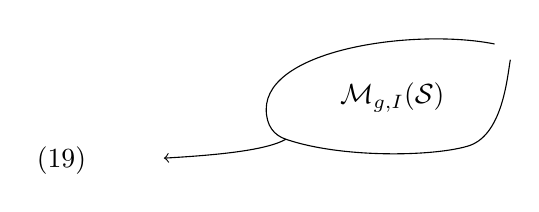
\begin{tikzpicture}[baseline=(m.base)]
\node (m) at (0,0) {$\mathcal M_{g,I}(\mathcal S)$};
\draw (1.3,.68) .. controls (.3,.88) and (-1.6,.62) .. (-1.6,-.15)
 .. controls (-1.6,-.36) and (-1.5,-.48) .. (-1.35,-.53)
 .. controls (-.65,-.77) and (.5,-.75) .. (.95,-.62)
 .. controls (1.4,-.5) and (1.46,.25) .. (1.5,.48);
\draw[->] (-1.35,-.53) .. controls (-1.6,-.67) and (-2.2,-.73) .. (-2.9,-.77);
\node at (-4.2,-.8) {$(19)$};
\end{tikzpicture}}
le \deleted{\unsure{catégorie|catég.}}\inserted{groupoïde} des courbes relatives $Y$ (propres, lisses, $0$-connexes) sur $\mathcal S$, \uline{$I$-ponctuées} i.e. munies d'un mono $I_{\mathcal S}\hookrightarrow Y$. On trouve donc, si
\[
(20)\qquad\mathcal M_G(\mathcal S)
\]
désigne le groupoïde des courbes standart $G$-épinglées sur $\mathcal S$, une équivalence
\[
(21)\qquad\mathcal M_G(\mathcal S)\approxeq\prod_{\alpha\in S}\mathcal M_{g_\alpha,\widehat I_\alpha}(\mathcal S).
\]
\mspage{18}

\scanpage{21}
\unsure{correspondante|correspondants}, \deleted{\unsure{qui|que}} de sorte qu'on aura un iso can.
\margin{plutôt, une \uline{équivalence}}
\[
(23)\qquad\mathcal M_{\unsure{G}}\simeq\prod_\alpha\mathcal M_{g_\alpha,\widehat I_\alpha}.
\]
Notons que $\Gamma=\operatorname{Aut}G$ opère sur $\mathcal M_G$ de façon évidente, et aussi sur le système $(\widehat I_\alpha,g_\alpha)_{\alpha\in S}$ donc sur le deuxième mb de (23), qui est un iso. compatible aux op. de $\Gamma$.

On peut considérer la multiplicité mixte
\[
(24)\qquad(\mathcal M_G,\Gamma)=\mathcal M_{[G]},
\]
qui a priori ne dépend que du type d'isomorphie $[G]$ de $G$, et qui s'interprète, en termes de ce dernier, comme la multiplicité schématique modulaire pour \unsure{le|les|la} groupoïde fibré (sur la $2$-cat. des multiplicités schématiques) des courbes standart relatives de type $[G]$.
% Light lower-edge pagination; hand unidentified.
\mspage{20}

\scanpage{22}
\mspage{10}
\margin{$(g,\nu=\operatorname{card}J)$ anabélien}
\uline{NB} Si $\operatorname{card}J=\nu$, alors $M_{g,J}$ est isomorphe au schéma modulaire $M^!_{g,\nu}$ (via un iso. $[1,\nu]\cap\mathbb Z\simeq J$), de façon compatible avec les autom. des groupes $\unsure{\mathfrak S_J|\mathfrak G_J|\mathcal G_J}$ et $\unsure{\mathfrak S_\nu|\mathfrak G_\nu|\mathcal G_\nu}$. On sait que $M^!_{g,\nu}$ est lisse de type fini sur $\mathbb Z$. Il en est donc de $\bar m$ \unsure{des|de} $M_{g,J}$, donc aussi de $M_G$ (pour $G$ semi-stable) et de $M_{[G]}=(M_G,\Gamma)$.

4. \uline{La théorie de Mumford}-\uline{Deligne}

Soient $\mathcal S$ une multiplicité schématique, $\mathfrak X$ une \deleted{courbe} schéma relatif sur $\mathcal S$, propre sur $\mathcal S$, $\underline I$ un sous-schéma fermé de $\mathfrak X$. On dit que $(\mathfrak X,\underline I)$ est une MD-courbe relative sur $\mathcal S$, si $\mathfrak X,\underline I$ sont plats de présentation finie sur $\mathcal S$, et si pour tt pt géom. de $\mathcal S$, \unsure{la|le}
\mspage{21}

\scanpage{23}
fibre $(\mathfrak X_{\bar s},\underline I_{\bar s})$ est une \inserted{MD-}courbe géométrique sur $k(s)$ -- i.e. $\mathfrak X_{\bar s}$ est $0$-connexe, de dim $1$, \deleted{\unsure{ainsi q.}} les pts singuliers sont \inserted{$\notin I_{\bar s}$ et sont} des pts doubles ordinaires, et enfin la condition de rigidité infinitésimale \inserted{(en \unsure{autismes|conditions})} est satisfaite -- \deleted{donc} i.e. on exige que $\mathfrak X_{\bar s}$ ne soit pas de genre $1$ lisse avec $I_{\bar s}=\unsure{\phi|\varnothing}$, et que les comp. irréd. de genre $0$ de $\mathfrak X_{\bar s}$ soient de ``poids marqué''
\[
\geqslant 3.
\]
La différence avec les considérations du n° précédent, c'est que maintenant ($\bar m$ sur une base $\mathcal S$ connexe, p.ex. \deleted{$\unsure{\mathcal S=}$} un trait) les \uline{types} des fibres géométriques peuvent varier d'un pt géom. à un autre. Mais il est clair que le type \uline{numérique} $(g,\nu)$ ne change pas (invariance \unsure{des|de} $\chi(\widehat X_s,\underline O_{\widehat X_s})\ldots$ et de $\operatorname{card}\underline I_s$), plus précisément,
% Two clipped right-edge ink fragments; wording and extent unrecoverable.
% Lower fragment is crossed; its deletion state remains less than certain.
\margin{\illegible{1}\ \deleted{\illegible{1}}}
% Light lower-edge pagination; hand unidentified.
\mspage{22}
